\newpage
\section{CNN Architectures}
\subsection{Case Studies}
\subsubsection{AlexNet}
\begin{figure}[!htb]
    \centering
    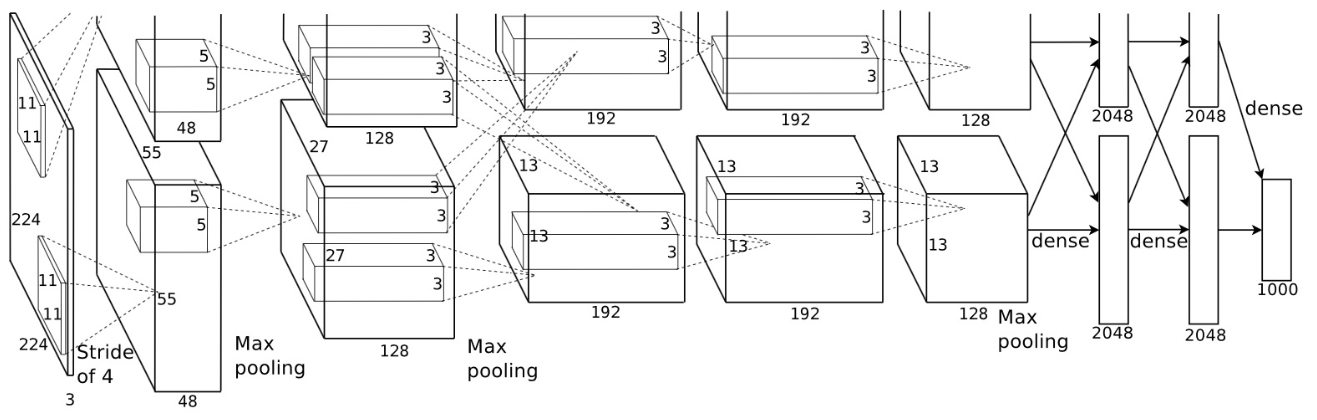
\includegraphics[width=0.42\textwidth]{pic/Lec9/AlexNet.png}
    \caption{AlexNet}
\end{figure}
通信网络

\textbf{Architecture}: Input $[227\times 227\times 3]$
\begin{enumerate}
    \item CONV1: 96 filters $11\times 11$ applied at stride 4, pad 0 
    \subitem Output volume: $[55\times 55\times 96]$
    \item MAX POOL1: $3\times3$ filters applied at stride 2
    \subitem Output volume: $[27\times 27\times 96]$
    \item NORM1
    \item CONV2: 256 filters $5\times 5$ applied at stride 1, pad 2 
    \subitem Output volume: $[27\times 27\times 256]$
    \item MAX POOL2: filters $3\times 3$ applied at stride 2
    \subitem Output volume: $[13\times 13\times 256]$
    \item NORM2
    \item CONV3: 384 filters $3\times 3$ applied at stride 1, pad 1
    \subitem Output volume: $[13\times 13\times 384]$
    \item CONV4: 384 filters $3\times 3$ applied at stride 1, pad 1 
    \subitem Output volume: $[13\times 13\times 384]$
    \item CONV5: 256 filters $3\times 3$ applied at stride 1, pad 1 
    \subitem Output volume: $[13\times 13\times 256]$
    \item Max POOL3: filters $3\times 3$ applied at stride 2
    \subitem Output volume: $[6\times 6\times 256]$
    \item FC6: 4096 neurons
    \subitem Output volume: $[4096]$
    \item FC7: 4096 neurons
    \subitem Output volume: $[4096]$
    \item FC8: 1000 neurons
    \subitem Output volume: $[1000]$
\end{enumerate}


\subsubsection{VGG}
Small filters, Deeper networks. 

小卷积核的堆叠感受野可以等效于大卷积核. 
\begin{figure}[!htb]
    \centering
    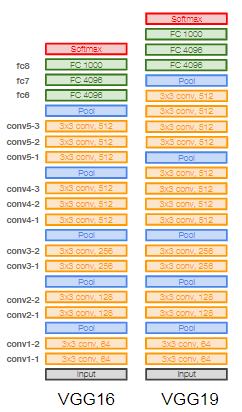
\includegraphics[width=0.12\textwidth]{pic/Lec9/VGG.png}
    \caption{VGG}
\end{figure}



\subsubsection{GoogLeNet}
参数较少.
\begin{figure}[!htb]
    \centering
    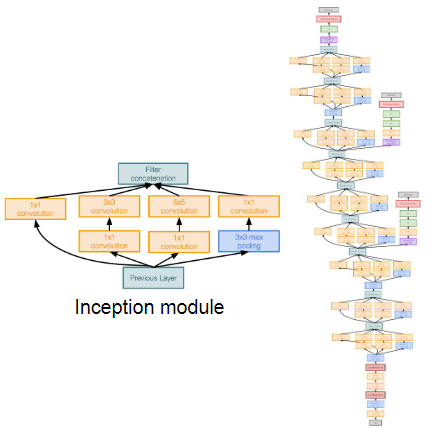
\includegraphics[width=0.309\textwidth]{pic/Lec9/GoogLeNet.png}
    \caption{GoogLeNet}
\end{figure}
平行使用多个filter操作并将他们整合. 但复杂度高. 使用 $1\times1$ conv 来改变特征维度以减少计算. 

因为太深了, 所以在中间增加了输出以更早的给出梯度. 


\subsubsection{ResNet}
使用残差链接构建的极深的网络


单纯加深网络层数, 会让模型表现变差, 且不是由于过拟合造成的. 

假设: 这是个优化问题, 更深的模型更难以优化. 

解决方案: 所以只优化增量以降低优化难度(直觉, 没有证明). $H(x)=F(x)+x$.  Use layers to
fit residual $F(x) = H(x) - x$ instead of $H(x)$ directly. 

\begin{figure}[!htb]
    \centering
    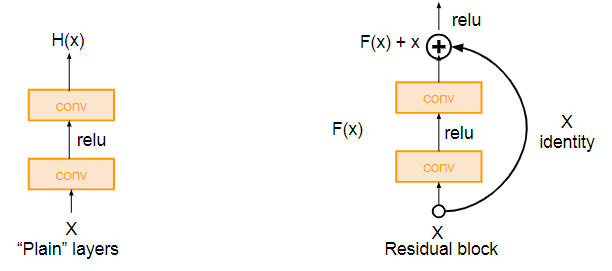
\includegraphics[width=0.309\textwidth]{pic/Lec9/Residual block}
    \caption{Residual}
\end{figure}

\subsection{Other architectures}
\subsubsection{NiN (Network in Network)}
卷积层配合MLP. 

\begin{figure}[!htb]
    \centering
    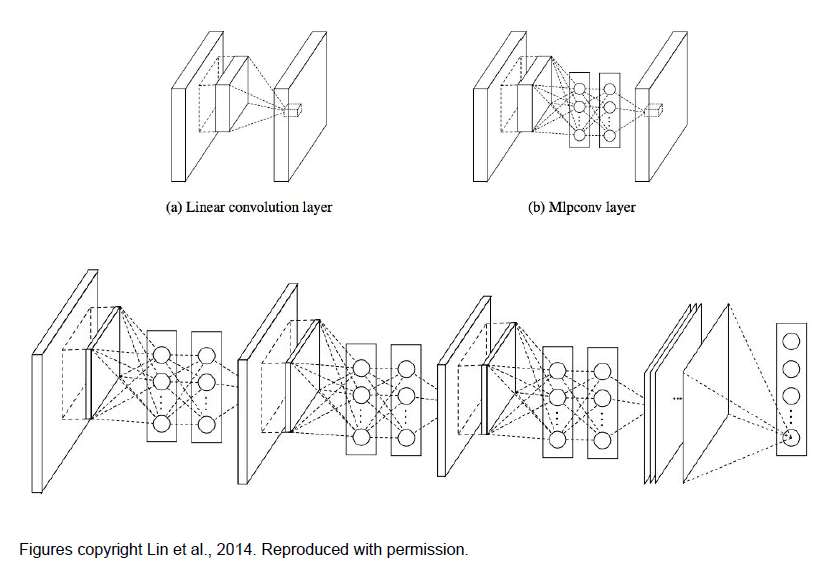
\includegraphics[width=0.309\textwidth]{pic/Lec9/NiN.png}
    \caption{NiN}
\end{figure}

\subsubsection{Wide ResNet}
更多的卷积层. 
\begin{figure}[!htb]
    \centering
    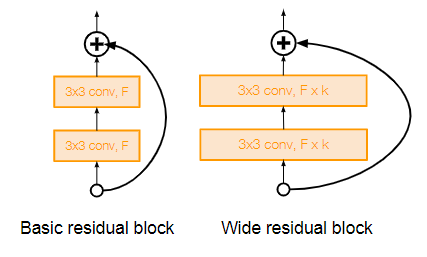
\includegraphics[width=0.309\textwidth]{pic/Lec9/Wide ResNet}
    \caption{Wide ResNet}
\end{figure}

\subsubsection{ResNeXT}
使用平行卷积提升宽度. 

\begin{figure}[!htb]
    \centering
    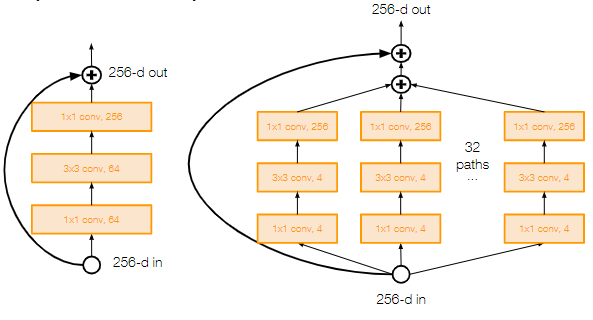
\includegraphics[width=0.309\textwidth]{pic/Lec9/ResNeXT}
    \caption{ResNeXT}
\end{figure}

